\chapter{Overview of Clinical Data Science {\color{red} DRAFT} \label{chapter:overview}}

The term ``data science'' has been overused in recent years, and it has become something of a buzzword as a result\footnote{See also: ``artificial intelligence'', ``machine learning'', ``deep learning''.}. However, I think it can best be described as: 
\begin{quote}
\textbf{data science}: Any endeavor in which statistics, machine learning, data analysis, computer science, and information science intersect with domain knowledge.
\end{quote}
Data science is about using the machinery of statistics and computer science to solve real-world problems. In the clinical domain, that means incorporating methods from epidemiology, biostatistics, computer science, and machine learning with insights gained from the clinical research literature and the practical experiences of physicians, nurses, hospital administrators, operational teams, and biomedical researchers.

So why is data science considered its own thing, and why am I creating a separate course about it instead of pointing you to Khan Academy, Coursera, etc., all of which have excellent courses on these various technical domains? Because (a) if you tried to learn data science that way, you'd never get anywhere; there are simply too many different subjects you'd have to master, and (b) clinical data has issues that are domain-specific, and that rarely come up in general courses on machine learning and related topics. Many times I will think I know what method to use to solve a particular problem, but then when it comes time to gather the data, unusual and unforeseen problems arise. This happens all the time to all of the biomedical and clinical data science researchers I know, and it is particularly problematic for people who are encountering data analysis and statistical/machine learning methods for the first time. Many assume the problem is them and give up, when in reality they are encountering a genuine difficulty with the data they're working with that the folks doing ad recommendations at Google never have to face.

However, my main reason for doing this is that I believe clinical and operational teams will increasingly come to rely on data, and that the people on those teams who can confidently interact with data will be our future leaders. And I'd like those people to be you.

%%%%%%%%%%%%%%%%%%%%%%%%%%%%%%%%%%%%%%%%%%%%%%%%%%%%%%%%%%%%%%%%%%%%%%%%%%%%%%%%

\section{Project Examples}

Whenever I teach, I ask students to provide some examples of projects for which they think data and machine learning/statistics could be useful. The following are real examples. There are many and some of them are long, but I encourage you to read through all of them to see the diversity of problems that physicians and folks working in population health, health system operations, etc. come up with.

\begin{enumerate}
\item \textit{Unnecessary ER trips.} ``Given a number of factors (types of admissions a person has had in the past, number of admissions/re-admissions, social determinants, etc.) can we predict who is going to show up at the emergency room unnecessarily''
\item \textit{Good/poor candidates for program.} ``determine if patients are good or poor candidates for one of our specialty care model bundle programs''
\item \textit{Predicting unplanned admissions.} ``predicting unplanned inpatient admissions based on many different variables (e.g. chronic conditions, engagement with primary care, etc.) and how these inputs interact with each other''
\item \textit{Recommending an intervention.} ``\dots stratification/prioritization of care management or other interventions or for clinical decision support\dots a tool would recommend an appropriate intervention based on the profile of the patient''
\item \textit{Recommending a diagnosis.} ``Based on unstructured chat conversations and also structured questions/forms/data\dots map out possible care pathways. For example, if someone says they have stomach pain, gives their zip code, insurance, pain tolerance and symptoms, and is logged in so we have past history, ask a few more questions and then we could determine they are 45\% likely to have ulcer vs. constipation vs. food poisoning vs. appendicitis.''
\item \textit{Predicting the amount paid by patients.} ``Patient bill estimates - learning from claims data typical amount paid by patients for appointment reasons/types (e.g. estimate of additional services/care administered, and associated cost, based on patient details such as age, gender, etc.)''
\item \textit{Identifying patient subtypes.} ``identify cohorts within a population with chronic conditions based on their differences in longitudinal care across the continuum of settings (inpatient, ambulatory, primary care, specialty care, etc.)''
\item \textit{Which conversations are similar?} ``using previous chat histories to train (a chatbot) and become more effective/efficient for different, future patient chat experiences''
\item \textit{Predictors of COVID-19 outcomes.} ``Get baseline diabetes control marker (HbA1C) and acute glycemic control (inpatient glucose values) and see if either is a stronger predictor of COVID-19 outcomes (ICU, intubation, death).''
\item \textit{Factors influencing mortality in myelofibrosis.} ``We see lots of patients who are ineligible for clinical trials based on comorbidities and underlying organ dysfunction. However it is unclear how these factors affect OS. I would like to extract comorbidity data and baseline laboratory factors in patients with myelofibrosis to see how these factors affect mortality, if controlled for such important factors such as treatment, age, sex, insurance, number of comorbidities, and clinical risk score (DIPSS).''
\item \textit{Non-adherence and difficult-to-treat asthma.} ``We want to see whether non-adherence to prescribed inhaled corticosteroids plays a major role in poorly controlled asthma. Difficult-to-treat asthma can be evaluated by the number of ED visits, hospitalizations, prescriptions of prednisone and prescriptions of biological therapies. Using EPIC [we] can obtain medicine reconciliation information, of prescriptions sent, what proportion of those prescriptions were dispensed by Pharmacy. Question is can we find associations between the percentage of prescriptions filled and difficult-to-treat asthma.''
\item \textit{Impact of diabetes and hyperglycemia on progression-free survival.} ``Aim: Assess the impact of diabetes and hyperglycemia on first-line systemic therapy response (progression-free survival) in patients with advanced non-small cell lung cancer. Diabetes- defined by presence of diagnosis codes coding for diabetes. Hyperglycemia- random glucose >200 ng/dL. Covariates of interest- age, sex, other treatments (RT, surgery), malignancy characteristics (stage, histology), smoking history, ecog (performance status), comorbidities, medications (steroids, anti-hyperglycemics)''
\item \textit{Effect of statin use on MACE.} ``Retrospective cohort study in elderly patients with CAD taking statins\dots exposed group are patients on a high-intensity statin; control group are patients on a moderate- or low-intensity statin. Participants matched based on age, gender, LDL category, and Elixhauser index category\dots The primary efficacy outcome would be the time-to-first-event of 3-point MACE\footnote{MACE stands for ``Major Adverse Cardiac Event''. The 3-point MACE is a composite of nonfatal stroke, nonfatal myocardial infarction, and cardiovascular death.}.''
\item \textit{Clustering patients with NAFLD.} ``We wanted to understand non-alcoholic fatty liver disease (NAFLD) better, so we developed a cohort of NAFLD patients using EMR-based criteria and then clustered them based on co-morbidities, medications, vital signs, and lab values to identify NAFLD subtypes. We then characterized the phenotypes and outcomes of the different subtypes.''
\end{enumerate}

%%%%%%%%%%%%%%%%%%%%%%%%%%%%%%%%%%%%%%%%%%%%%%%%%%%%%%%%%%%%%%%%%%%%%%%%%%%%%%%%

\section{A Taxonomy of Problems}

All of these examples describe situations where we want to use data to answer questions of clinical or operational importance. While the details differ in each scenario, the important thing to notice here is that many of the tasks themselves are structurally similar. 

For example, all of the items except $7-8$ and $14$ describe situations where we want to associate information about a patient with a particular outcome or recommendation. Using information about a patient to estimate the size of a bill (\#6) may appear to be a very different problem than uncovering factors influencing myelofibrosis mortality (\#10), but the structure of the two problems is similar: the patient features are used as input, and the output is whatever quantity you care about (e.g. the cost to the patient in dollars or the probability of mortality by a certain timepoint). 

Learning to see these types of similarities will give you a tremendous amount of power when attacking new problems in clinical data science. It will allow you to confidently deploy methods you used to solve one problem on a wide range of other problems. Each new method you learn then multiplies your capacity to solve problems, rather than adding to it. 

\begin{question}{}
How are items $7-8$ and $14$ different from the rest? 
% supervised vs. unsupervised learning
\end{question}

\begin{question}{}
How are items $1-6$ similar to items $9-13$ and how are they different? 
% all supervised learning, but in the first case just interested in prediction
% in the second case, interested in isolating the effect(s) of specific factor(s)
\end{question}

\begin{question}{}
How do items $1-3$ differ from items $4-5$ and how are they similar? 
% binary vs. multi-class classification
\end{question}

\begin{question}{}
How do items $1-3$ differ from item $6$? How is item $6$ different from all of the other items? 
% classification vs. regression
\end{question}

\begin{question}{}
How do items $9-11$ differ from items $12-13$? 
% classification vs. time-to-event outcome (survival analysis)
\end{question}

%%%%%%%%%%%%%%%%%%%%%%%%%%%%%%%%%%%%%%%%%%%%%%%%%%%%%%%%%%%%%%%%%%%%%%%%%%%%%%%%

\section{Terms and Contrasts}

The basic ways in which clinical data science problems vary fall into a few broad categories. These categories encompass concepts from both traditional clinical disciplines, like epidemiology, and machine learning/statistics.

\subsection{Observational Study vs. Experiment}

Observational is where you observe certain variables and try to determine if there is any correlation. Experimental is where you control certain variables and try to determine if there is any causality.

Here is the NIH's definition of a \textbf{clinical trial}:
\begin{quote}
A research study in which one or more human subjects are prospectively assigned to one or more interventions (which may include placebo or other control) to evaluate the effects of those interventions on health-related biomedical or behavioral outcomes.
\end{quote}
We can think of a clinical trial, therefore, as an experiment in which we control the intervention. 

\subsection{Prospective vs. Retrospective}



\subsection{Supervised vs. Unsupervised Learning}

This distinction, most often found in discussions of machine learning, refers to the way in which training data is applied to solve a problem. In \textbf{supervised learning}, the training data consist of pairs of input features and labels, and the algorithm learns to predict the value of the label from the input features. The general setup for supervised learning looks like this:
\begin{center}
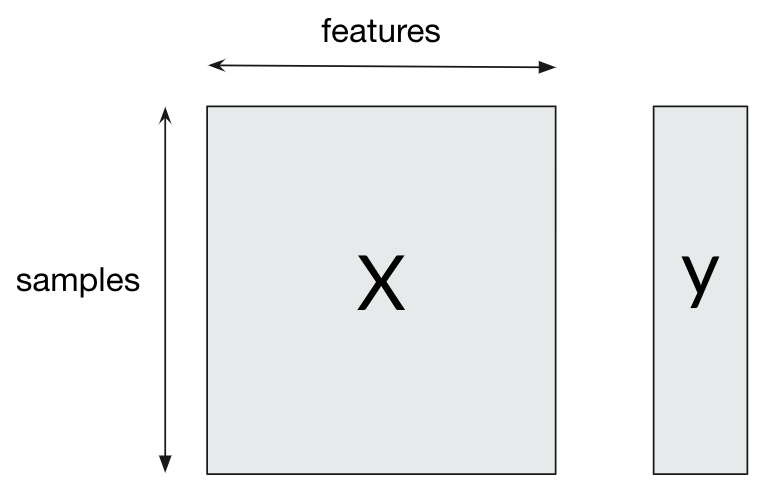
\includegraphics[width=0.7\textwidth]{img/supervised-learning.png}
\end{center}

In \textbf{unsupervised learning}, only the input features are present and the algorithm learns to recognize patterns or structure in the inputs. The general setup for unsupervised learning looks like this:
\begin{center}
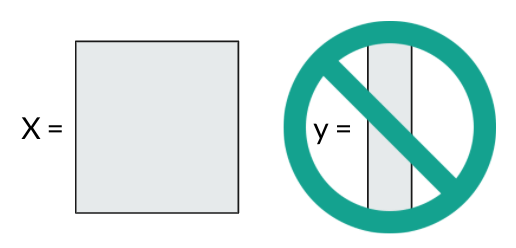
\includegraphics[width=0.7\textwidth]{img/unsupervised-learning-diagram.png}
\end{center}

There are also two other types of machine learning. In \textbf{semi-supervised learning}, a small amount of labeled data is used to create a much larger, weakly-labeled set of training data that is then fed to a supervised learning algorithm. In \textbf{reinforcement learning}, an algorithm is trained with a reward system which provides feedback on the quality of the action the system performs in a given situation instead of (as in supervised learning) simply providing the ``right answer''. 

%%%%%%%%%%%%%%%%%%%%%%%%%%%%%%%%%%%%%%%%%%%%%%%%%%%%%%%%%%%%%%%%%%%%%%%%%%%%%%%%




 

